\documentclass[twoside]{book}

% Packages required by doxygen
\usepackage{fixltx2e}
\usepackage{calc}
\usepackage{doxygen}
\usepackage[export]{adjustbox} % also loads graphicx
\usepackage{graphicx}
\usepackage[utf8]{inputenc}
\usepackage{makeidx}
\usepackage{multicol}
\usepackage{multirow}
\PassOptionsToPackage{warn}{textcomp}
\usepackage{textcomp}
\usepackage[nointegrals]{wasysym}
\usepackage[table]{xcolor}

% Font selection
\usepackage[T1]{fontenc}
\usepackage[scaled=.90]{helvet}
\usepackage{courier}
\usepackage{amssymb}
\usepackage{sectsty}
\renewcommand{\familydefault}{\sfdefault}
\allsectionsfont{%
  \fontseries{bc}\selectfont%
  \color{darkgray}%
}
\renewcommand{\DoxyLabelFont}{%
  \fontseries{bc}\selectfont%
  \color{darkgray}%
}
\newcommand{\+}{\discretionary{\mbox{\scriptsize$\hookleftarrow$}}{}{}}

% Page & text layout
\usepackage{geometry}
\geometry{%
  a4paper,%
  top=2.5cm,%
  bottom=2.5cm,%
  left=2.5cm,%
  right=2.5cm%
}
\tolerance=750
\hfuzz=15pt
\hbadness=750
\setlength{\emergencystretch}{15pt}
\setlength{\parindent}{0cm}
\setlength{\parskip}{3ex plus 2ex minus 2ex}
\makeatletter
\renewcommand{\paragraph}{%
  \@startsection{paragraph}{4}{0ex}{-1.0ex}{1.0ex}{%
    \normalfont\normalsize\bfseries\SS@parafont%
  }%
}
\renewcommand{\subparagraph}{%
  \@startsection{subparagraph}{5}{0ex}{-1.0ex}{1.0ex}{%
    \normalfont\normalsize\bfseries\SS@subparafont%
  }%
}
\makeatother

% Headers & footers
\usepackage{fancyhdr}
\pagestyle{fancyplain}
\fancyhead[LE]{\fancyplain{}{\bfseries\thepage}}
\fancyhead[CE]{\fancyplain{}{}}
\fancyhead[RE]{\fancyplain{}{\bfseries\leftmark}}
\fancyhead[LO]{\fancyplain{}{\bfseries\rightmark}}
\fancyhead[CO]{\fancyplain{}{}}
\fancyhead[RO]{\fancyplain{}{\bfseries\thepage}}
\fancyfoot[LE]{\fancyplain{}{}}
\fancyfoot[CE]{\fancyplain{}{}}
\fancyfoot[RE]{\fancyplain{}{\bfseries\scriptsize Generated by Doxygen }}
\fancyfoot[LO]{\fancyplain{}{\bfseries\scriptsize Generated by Doxygen }}
\fancyfoot[CO]{\fancyplain{}{}}
\fancyfoot[RO]{\fancyplain{}{}}
\renewcommand{\footrulewidth}{0.4pt}
\renewcommand{\chaptermark}[1]{%
  \markboth{#1}{}%
}
\renewcommand{\sectionmark}[1]{%
  \markright{\thesection\ #1}%
}

% Indices & bibliography
\usepackage{natbib}
\usepackage[titles]{tocloft}
\setcounter{tocdepth}{3}
\setcounter{secnumdepth}{5}
\makeindex

% Custom commands
\newcommand{\clearemptydoublepage}{%
  \newpage{\pagestyle{empty}\cleardoublepage}%
}

\usepackage{caption}
\captionsetup{labelsep=space,justification=centering,font={bf},singlelinecheck=off,skip=4pt,position=top}

%===== C O N T E N T S =====

\begin{document}

% Titlepage & ToC
\pagenumbering{alph}
\begin{titlepage}
\vspace*{7cm}
\begin{center}%
{\Large qumbia-\/client \\[1ex]\large 1.\+x }\\
\vspace*{1cm}
{\large Generated by Doxygen 1.8.14}\\
\end{center}
\end{titlepage}
\clearemptydoublepage
\pagenumbering{roman}
\tableofcontents
\clearemptydoublepage
\pagenumbering{arabic}

%--- Begin generated contents ---
\chapter{Main Page}
\label{index}{\itshape cumbia-\/epics} is the cumbia module for the {\tt Experimental Physics and Industrial Control System} (E\+P\+I\+CS) control system.\section{Related readings}\label{index_related_readings}
\subsection{Tutorials}\label{index_tutorials}
\tabulinesep=1mm
\begin{longtabu} spread 0pt [c]{*{2}{|X[-1]}|}
\hline
\rowcolor{\tableheadbgcolor}\textbf{ Tutorials  }&\textbf{ Module   }\\\cline{1-2}
\endfirsthead
\hline
\endfoot
\hline
\rowcolor{\tableheadbgcolor}\textbf{ Tutorials  }&\textbf{ Module   }\\\cline{1-2}
\endhead
{\tt Writing a {\itshape cumbia} activity}  &{\tt cumbia}   \\\cline{1-2}
{\tt Writing an activity}  &{\tt cumbia-\/tango}   \\\cline{1-2}
{\tt Cu\+Data for Tango}  &{\tt cumbia-\/tango}   \\\cline{1-2}
{\tt Writing a Qt widget that integrates with cumbia}  &{\tt qumbia-\/tango-\/controls}   \\\cline{1-2}
{\tt Using {\itshape cumbia ui make}} to process Qt designer UI files  &{\tt qumbia-\/apps/cuuimake}   \\\cline{1-2}
{\tt Writing a {\itshape Qt application} with cumbia and Tango}.  &{\tt qumbia-\/apps/qumbiaprojectwizard}   \\\cline{1-2}
{\tt Porting a {\itshape Q\+Tango application} to {\itshape cumbia-\/tango}}.  &{\tt qumbia-\/apps/qumbiaprojectwizard}   \\\cline{1-2}
{\tt {\itshape cumbia new control}}\+: quickly add a custom Qt widget to a cumbia project  &{\tt qumbia-\/apps/qumbianewcontrolwizard}   \\\cline{1-2}
{\tt Understanding {\itshape cumbia-\/qtcontrols constructors, sources and targets}}  &{\tt cumbia-\/qtcontrols}.   \\\cline{1-2}
\end{longtabu}
\subsection{Modules}\label{index_cumodules}
\tabulinesep=1mm
\begin{longtabu} spread 0pt [c]{*{1}{|X[-1]}|}
\hline
\rowcolor{\tableheadbgcolor}\textbf{ Other {\itshape cumbia} modules   }\\\cline{1-1}
\endfirsthead
\hline
\endfoot
\hline
\rowcolor{\tableheadbgcolor}\textbf{ Other {\itshape cumbia} modules   }\\\cline{1-1}
\endhead
{\tt cumbia module}.   \\\cline{1-1}
{\tt cumbia-\/tango module}.   \\\cline{1-1}
{\tt cumbia-\/qtcontrols module}.   \\\cline{1-1}
{\tt cumbia-\/qtcontrols module}.   \\\cline{1-1}
{\tt qumbia-\/epics module}.   \\\cline{1-1}
{\tt qumbia-\/epics-\/controls module}.   \\\cline{1-1}
\end{longtabu}
\subsection{apps}\label{index_cu_apps}
These applications (and their documentation, that has already been mentioned in the {\itshape Tutorials} table above) must be installed from the {\itshape qumbia-\/apps} sub-\/directory of the {\itshape cumbia-\/libs} distribution. To install them, {\itshape cd} into that folder and execute\+:


\begin{DoxyCode}
qmake
make
sudo make install
\end{DoxyCode}


Along the applications executables and documentation, two bash scripts will be installed\+:


\begin{DoxyItemize}
\item /etc/bash\+\_\+completion.d/cumbia
\item /etc/bash/bashrc.d/cumbia.\+sh
\end{DoxyItemize}

They define shortcuts for the common operations provided by the {\itshape qumbia-\/apps} applications as follows\+:

\tabulinesep=1mm
\begin{longtabu} spread 0pt [c]{*{3}{|X[-1]}|}
\hline
\rowcolor{\tableheadbgcolor}\textbf{ Applications (command line)  }&\textbf{ description  }&\textbf{ app   }\\\cline{1-3}
\endfirsthead
\hline
\endfoot
\hline
\rowcolor{\tableheadbgcolor}\textbf{ Applications (command line)  }&\textbf{ description  }&\textbf{ app   }\\\cline{1-3}
\endhead
{\itshape cumbia new project}  &create a new cumbia project  &{\tt qumbia-\/apps/qumbiaprojectwizard}   \\\cline{1-3}
{\itshape cumbia import}  &migrate a Q\+Tango project into cumbia  &{\tt qumbia-\/apps/qumbiaprojectwizard}   \\\cline{1-3}
{\itshape cumbia new control}  &write a {\itshape cumbia control} reader or writer  &{\tt qumbia-\/apps/qumbianewcontrolwizard}   \\\cline{1-3}
{\itshape cumbia ui make}  &run {\itshape cuuimake} to generate {\itshape qt+cumbia} ui\+\_\+$\ast$.h files  &{\tt qumbia-\/apps/cuuimake}   \\\cline{1-3}
{\itshape cumbia client}  &run a generic cumbia client  &{\tt qumbia-\/apps/cumbia\+\_\+client}   \\\cline{1-3}
\end{longtabu}


{\itshape bash auto completion} will help you use these shortcuts\+: try


\begin{DoxyCode}
cumbia <TAB>
\end{DoxyCode}


or


\begin{DoxyCode}
cumbia new <TAB>
\end{DoxyCode}


At the moment {\bfseries only a monitor (reader) has been implemented}.

\begin{DoxyParagraph}{Example}
In the qumbia-\/epics-\/controls module, under the {\itshape examples} directory, you will find an example of \doxyref{Cumbia\+Epics}{p.}{classCumbiaEpics} usage. It is completely equivalent to the {\itshape cumbia/tango} counterpart.
\end{DoxyParagraph}
See {\tt qumbia-\/epics-\/controls} documentation. 
\chapter{Hierarchical Index}
\section{Class Hierarchy}
This inheritance list is sorted roughly, but not completely, alphabetically\+:\begin{DoxyCompactList}
\item \contentsline{section}{Cu\+Action\+Factory\+Service\+Private}{\pageref{classCuActionFactoryServicePrivate}}{}
\item Cu\+Continuous\+Activity\begin{DoxyCompactList}
\item \contentsline{section}{Cu\+Monitor\+Activity}{\pageref{classCuMonitorActivity}}{}
\end{DoxyCompactList}
\item \contentsline{section}{Cu\+Ep\+Config\+Activity\+Private}{\pageref{classCuEpConfigActivityPrivate}}{}
\item \contentsline{section}{Cu\+Epics\+Action\+FactoryI}{\pageref{classCuEpicsActionFactoryI}}{}
\begin{DoxyCompactList}
\item \contentsline{section}{Cu\+Epics\+Att\+Conf\+Factory}{\pageref{classCuEpicsAttConfFactory}}{}
\item \contentsline{section}{Cu\+Epics\+Reader\+Factory}{\pageref{classCuEpicsReaderFactory}}{}
\item \contentsline{section}{Cu\+Epics\+Writer\+Factory}{\pageref{classCuEpicsWriterFactory}}{}
\end{DoxyCompactList}
\item \contentsline{section}{Cu\+Epics\+Read\+Options}{\pageref{classCuEpicsReadOptions}}{}
\item \contentsline{section}{Cu\+Epics\+World}{\pageref{classCuEpicsWorld}}{}
\item \contentsline{section}{Cu\+Epics\+World\+Config}{\pageref{classCuEpicsWorldConfig}}{}
\item \contentsline{section}{Cu\+Epics\+World\+Config\+Private}{\pageref{classCuEpicsWorldConfigPrivate}}{}
\item \contentsline{section}{Cu\+Epics\+World\+Private}{\pageref{classCuEpicsWorldPrivate}}{}
\item Cu\+Isolated\+Activity\begin{DoxyCompactList}
\item \contentsline{section}{Cu\+Ep\+Config\+Activity}{\pageref{classCuEpConfigActivity}}{}
\item \contentsline{section}{Cu\+Write\+Activity}{\pageref{classCuWriteActivity}}{}
\end{DoxyCompactList}
\item Cumbia\begin{DoxyCompactList}
\item \contentsline{section}{Cumbia\+Epics}{\pageref{classCumbiaEpics}}{}
\end{DoxyCompactList}
\item \contentsline{section}{Cu\+Monitor\+Activity\+Private}{\pageref{classCuMonitorActivityPrivate}}{}
\item \contentsline{section}{Cu\+Monitor\+Private}{\pageref{classCuMonitorPrivate}}{}
\item \contentsline{section}{Cu\+PV}{\pageref{structCuPV}}{}
\item Cu\+ServiceI\begin{DoxyCompactList}
\item \contentsline{section}{Cu\+Action\+Factory\+Service}{\pageref{classCuActionFactoryService}}{}
\item \contentsline{section}{Cu\+Ep\+C\+A\+Service}{\pageref{classCuEpCAService}}{}
\end{DoxyCompactList}
\item \contentsline{section}{Cu\+T\+Att\+Configuration\+Private}{\pageref{classCuTAttConfigurationPrivate}}{}
\item Cu\+Thread\+Listener\begin{DoxyCompactList}
\item \contentsline{section}{Cu\+Epics\+ActionI}{\pageref{classCuEpicsActionI}}{}
\begin{DoxyCompactList}
\item \contentsline{section}{Cu\+Ep\+Configuration}{\pageref{classCuEpConfiguration}}{}
\item \contentsline{section}{Cu\+Monitor}{\pageref{classCuMonitor}}{}
\item \contentsline{section}{Cu\+Put}{\pageref{classCuPut}}{}
\end{DoxyCompactList}
\end{DoxyCompactList}
\item \contentsline{section}{Cu\+T\+Writer\+Private}{\pageref{classCuTWriterPrivate}}{}
\item \contentsline{section}{Cu\+Write\+Activity\+Private}{\pageref{classCuWriteActivityPrivate}}{}
\item \contentsline{section}{Ep\+Source}{\pageref{classEpSource}}{}
\end{DoxyCompactList}

\chapter{Class Index}
\section{Class List}
Here are the classes, structs, unions and interfaces with brief descriptions\+:\begin{DoxyCompactList}
\item\contentsline{section}{\textbf{ Cu\+Action\+Factory\+Service} }{\pageref{classCuActionFactoryService}}{}
\item\contentsline{section}{\textbf{ Cu\+Action\+Factory\+Service\+Private} }{\pageref{classCuActionFactoryServicePrivate}}{}
\item\contentsline{section}{\textbf{ Cu\+Ep\+C\+A\+Service} }{\pageref{classCuEpCAService}}{}
\item\contentsline{section}{\textbf{ Cu\+Ep\+Config\+Activity} }{\pageref{classCuEpConfigActivity}}{}
\item\contentsline{section}{\textbf{ Cu\+Ep\+Config\+Activity\+Private} }{\pageref{classCuEpConfigActivityPrivate}}{}
\item\contentsline{section}{\textbf{ Cu\+Ep\+Configuration} }{\pageref{classCuEpConfiguration}}{}
\item\contentsline{section}{\textbf{ Cu\+Epics\+Action\+FactoryI} }{\pageref{classCuEpicsActionFactoryI}}{}
\item\contentsline{section}{\textbf{ Cu\+Epics\+ActionI} \\*Interface for an E\+P\+I\+CS {\itshape action}, as a reader (implemented) or a writer (not yet implemented) }{\pageref{classCuEpicsActionI}}{}
\item\contentsline{section}{\textbf{ Cu\+Epics\+Att\+Conf\+Factory} }{\pageref{classCuEpicsAttConfFactory}}{}
\item\contentsline{section}{\textbf{ Cu\+Epics\+Reader\+Factory} }{\pageref{classCuEpicsReaderFactory}}{}
\item\contentsline{section}{\textbf{ Cu\+Epics\+Read\+Options} }{\pageref{classCuEpicsReadOptions}}{}
\item\contentsline{section}{\textbf{ Cu\+Epics\+World} }{\pageref{classCuEpicsWorld}}{}
\item\contentsline{section}{\textbf{ Cu\+Epics\+World\+Config} \\*A class containing some configurations useful to several other objects }{\pageref{classCuEpicsWorldConfig}}{}
\item\contentsline{section}{\textbf{ Cu\+Epics\+World\+Config\+Private} }{\pageref{classCuEpicsWorldConfigPrivate}}{}
\item\contentsline{section}{\textbf{ Cu\+Epics\+World\+Private} }{\pageref{classCuEpicsWorldPrivate}}{}
\item\contentsline{section}{\textbf{ Cu\+Epics\+Writer\+Factory} }{\pageref{classCuEpicsWriterFactory}}{}
\item\contentsline{section}{\textbf{ Cumbia\+Epics} \\*Cumbia implementation over the E\+P\+I\+CS control system }{\pageref{classCumbiaEpics}}{}
\item\contentsline{section}{\textbf{ Cu\+Monitor} }{\pageref{classCuMonitor}}{}
\item\contentsline{section}{\textbf{ Cu\+Monitor\+Activity} }{\pageref{classCuMonitorActivity}}{}
\item\contentsline{section}{\textbf{ Cu\+Monitor\+Activity\+Private} }{\pageref{classCuMonitorActivityPrivate}}{}
\item\contentsline{section}{\textbf{ Cu\+Monitor\+Private} }{\pageref{classCuMonitorPrivate}}{}
\item\contentsline{section}{\textbf{ Cu\+Put} }{\pageref{classCuPut}}{}
\item\contentsline{section}{\textbf{ Cu\+PV} }{\pageref{structCuPV}}{}
\item\contentsline{section}{\textbf{ Cu\+T\+Att\+Configuration\+Private} }{\pageref{classCuTAttConfigurationPrivate}}{}
\item\contentsline{section}{\textbf{ Cu\+T\+Writer\+Private} }{\pageref{classCuTWriterPrivate}}{}
\item\contentsline{section}{\textbf{ Cu\+Write\+Activity} }{\pageref{classCuWriteActivity}}{}
\item\contentsline{section}{\textbf{ Cu\+Write\+Activity\+Private} }{\pageref{classCuWriteActivityPrivate}}{}
\item\contentsline{section}{\textbf{ Ep\+Source} }{\pageref{classEpSource}}{}
\end{DoxyCompactList}

\chapter{File Index}
\section{File List}
Here is a list of all files with brief descriptions\+:\begin{DoxyCompactList}
\item\contentsline{section}{\textbf{ cuepactionfactories.\+cpp} }{\pageref{cuepactionfactories_8cpp}}{}
\item\contentsline{section}{\textbf{ cuepactionfactories.\+h} }{\pageref{cuepactionfactories_8h}}{}
\item\contentsline{section}{\textbf{ cuepactionfactoryi.\+h} }{\pageref{cuepactionfactoryi_8h}}{}
\item\contentsline{section}{\textbf{ cuepactionfactoryservice.\+cpp} }{\pageref{cuepactionfactoryservice_8cpp}}{}
\item\contentsline{section}{\textbf{ cuepactionfactoryservice.\+h} }{\pageref{cuepactionfactoryservice_8h}}{}
\item\contentsline{section}{\textbf{ cuepactioni.\+cpp} }{\pageref{cuepactioni_8cpp}}{}
\item\contentsline{section}{\textbf{ cuepactioni.\+h} }{\pageref{cuepactioni_8h}}{}
\item\contentsline{section}{\textbf{ cuepcaservice.\+cpp} }{\pageref{cuepcaservice_8cpp}}{}
\item\contentsline{section}{\textbf{ cuepcaservice.\+h} }{\pageref{cuepcaservice_8h}}{}
\item\contentsline{section}{\textbf{ cuepconfigactivity.\+cpp} }{\pageref{cuepconfigactivity_8cpp}}{}
\item\contentsline{section}{\textbf{ cuepconfigactivity.\+h} }{\pageref{cuepconfigactivity_8h}}{}
\item\contentsline{section}{\textbf{ cuepconfiguration.\+cpp} }{\pageref{cuepconfiguration_8cpp}}{}
\item\contentsline{section}{\textbf{ cuepconfiguration.\+h} }{\pageref{cuepconfiguration_8h}}{}
\item\contentsline{section}{\textbf{ cuepics-\/world-\/config.\+cpp} }{\pageref{cuepics-world-config_8cpp}}{}
\item\contentsline{section}{\textbf{ cuepics-\/world-\/config.\+h} }{\pageref{cuepics-world-config_8h}}{}
\item\contentsline{section}{\textbf{ cuepics-\/world.\+cpp} }{\pageref{cuepics-world_8cpp}}{}
\item\contentsline{section}{\textbf{ cuepics-\/world.\+h} }{\pageref{cuepics-world_8h}}{}
\item\contentsline{section}{\textbf{ cuepreadoptions.\+cpp} }{\pageref{cuepreadoptions_8cpp}}{}
\item\contentsline{section}{\textbf{ cuepreadoptions.\+h} }{\pageref{cuepreadoptions_8h}}{}
\item\contentsline{section}{\textbf{ cumbiaepics.\+cpp} }{\pageref{cumbiaepics_8cpp}}{}
\item\contentsline{section}{\textbf{ cumbiaepics.\+h} }{\pageref{cumbiaepics_8h}}{}
\item\contentsline{section}{\textbf{ cumonitor.\+cpp} }{\pageref{cumonitor_8cpp}}{}
\item\contentsline{section}{\textbf{ cumonitor.\+h} }{\pageref{cumonitor_8h}}{}
\item\contentsline{section}{\textbf{ cumonitoractivity.\+cpp} }{\pageref{cumonitoractivity_8cpp}}{}
\item\contentsline{section}{\textbf{ cumonitoractivity.\+h} }{\pageref{cumonitoractivity_8h}}{}
\item\contentsline{section}{\textbf{ cuput.\+cpp} }{\pageref{cuput_8cpp}}{}
\item\contentsline{section}{\textbf{ cuput.\+h} }{\pageref{cuput_8h}}{}
\item\contentsline{section}{\textbf{ cuputactivity.\+cpp} }{\pageref{cuputactivity_8cpp}}{}
\item\contentsline{section}{\textbf{ cuputactivity.\+h} }{\pageref{cuputactivity_8h}}{}
\item\contentsline{section}{\textbf{ epsource.\+cpp} }{\pageref{epsource_8cpp}}{}
\item\contentsline{section}{\textbf{ epsource.\+h} }{\pageref{epsource_8h}}{}
\end{DoxyCompactList}

\chapter{Class Documentation}
\section{Element Class Reference}
\label{classElement}\index{Element@{Element}}


{\ttfamily \#include $<$element.\+h$>$}



Inheritance diagram for Element\+:\nopagebreak
\begin{figure}[H]
\begin{center}
\leavevmode
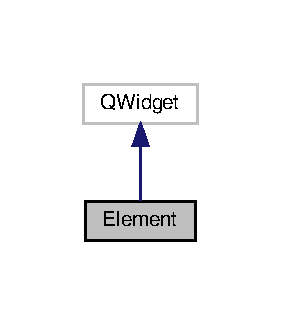
\includegraphics[width=135pt]{classElement__inherit__graph}
\end{center}
\end{figure}
\subsection*{Public Member Functions}
\begin{DoxyCompactItemize}
\item 
\textbf{ Element} (Q\+Widget $\ast$parent=nullptr)
\end{DoxyCompactItemize}


\subsection{Constructor \& Destructor Documentation}
\mbox{\label{classElement_a13abe7d029dbf66dac43fca1ae8f23ee}} 
\index{Element@{Element}!Element@{Element}}
\index{Element@{Element}!Element@{Element}}
\subsubsection{Element()}
{\footnotesize\ttfamily Element\+::\+Element (\begin{DoxyParamCaption}\item[{Q\+Widget $\ast$}]{parent = {\ttfamily nullptr} }\end{DoxyParamCaption})\hspace{0.3cm}{\ttfamily [explicit]}}



The documentation for this class was generated from the following files\+:\begin{DoxyCompactItemize}
\item 
\textbf{ element.\+h}\item 
\textbf{ element.\+cpp}\end{DoxyCompactItemize}

\input{classQumbiaClient}
\chapter{File Documentation}
\section{element.\+cpp File Reference}
\label{element_8cpp}\index{element.\+cpp@{element.\+cpp}}
{\ttfamily \#include \char`\"{}element.\+h\char`\"{}}\newline
Include dependency graph for element.\+cpp\+:
\nopagebreak
\begin{figure}[H]
\begin{center}
\leavevmode
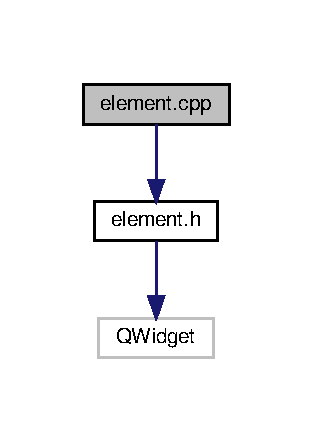
\includegraphics[width=150pt]{element_8cpp__incl}
\end{center}
\end{figure}

\section{element.\+h File Reference}
\label{element_8h}\index{element.\+h@{element.\+h}}
{\ttfamily \#include $<$Q\+Widget$>$}\newline
Include dependency graph for element.\+h\+:
\nopagebreak
\begin{figure}[H]
\begin{center}
\leavevmode
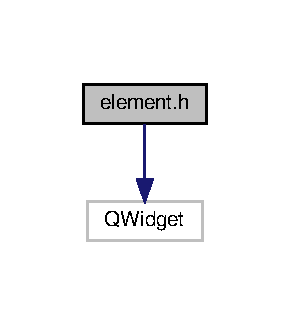
\includegraphics[width=139pt]{element_8h__incl}
\end{center}
\end{figure}
This graph shows which files directly or indirectly include this file\+:
\nopagebreak
\begin{figure}[H]
\begin{center}
\leavevmode
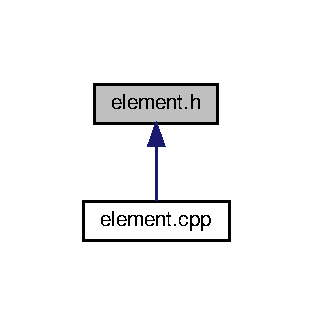
\includegraphics[width=150pt]{element_8h__dep__incl}
\end{center}
\end{figure}
\subsection*{Classes}
\begin{DoxyCompactItemize}
\item 
class \textbf{ Element}
\end{DoxyCompactItemize}

\section{main.\+cpp File Reference}
\label{main_8cpp}\index{main.\+cpp@{main.\+cpp}}
{\ttfamily \#include \char`\"{}qumbia-\/client.\+h\char`\"{}}\newline
{\ttfamily \#include $<$quapplication.\+h$>$}\newline
{\ttfamily \#include $<$cumbiapool.\+h$>$}\newline
{\ttfamily \#include $<$cuthreadfactoryimpl.\+h$>$}\newline
{\ttfamily \#include $<$cucontextactionbridge.\+h$>$}\newline
{\ttfamily \#include $<$qthreadseventbridgefactory.\+h$>$}\newline
Include dependency graph for main.\+cpp\+:
\nopagebreak
\begin{figure}[H]
\begin{center}
\leavevmode
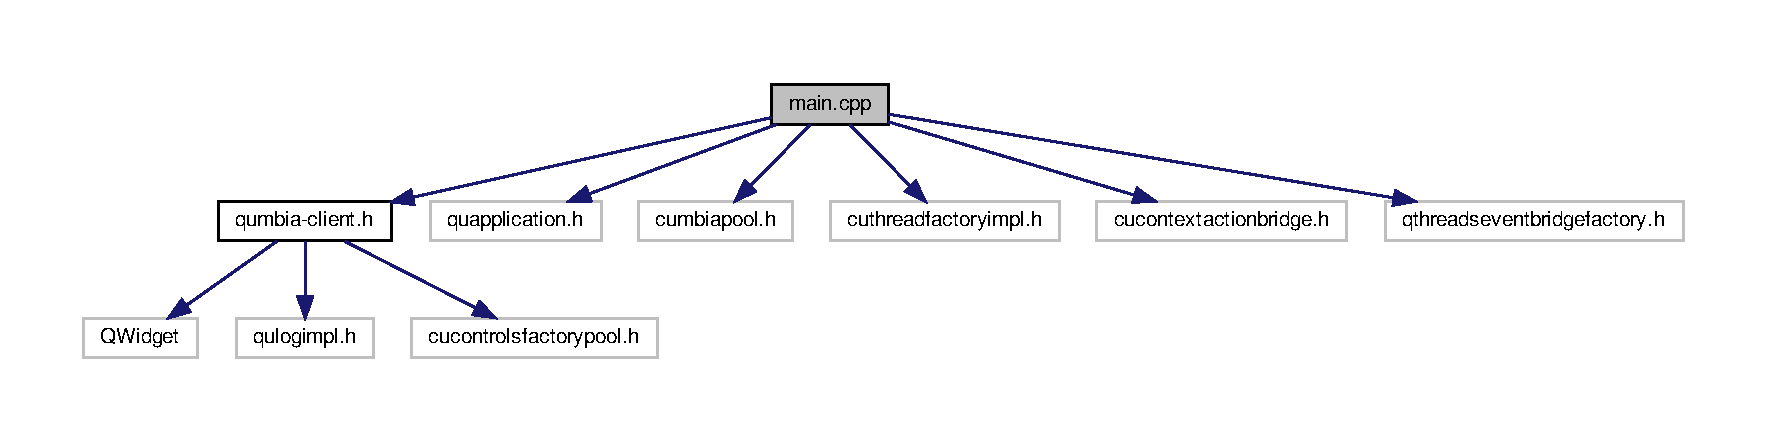
\includegraphics[width=350pt]{main_8cpp__incl}
\end{center}
\end{figure}
\subsection*{Functions}
\begin{DoxyCompactItemize}
\item 
int \textbf{ main} (int argc, char $\ast$argv[$\,$])
\end{DoxyCompactItemize}


\subsection{Function Documentation}
\mbox{\label{main_8cpp_a0ddf1224851353fc92bfbff6f499fa97}} 
\index{main.\+cpp@{main.\+cpp}!main@{main}}
\index{main@{main}!main.\+cpp@{main.\+cpp}}
\subsubsection{main()}
{\footnotesize\ttfamily int main (\begin{DoxyParamCaption}\item[{int}]{argc,  }\item[{char $\ast$}]{argv[$\,$] }\end{DoxyParamCaption})}


\input{qumbia-client_8cpp}
\input{qumbia-client_8h}
\section{ui\+\_\+cumbia\+\_\+client.\+h File Reference}
\label{ui__cumbia__client_8h}\index{ui\+\_\+cumbia\+\_\+client.\+h@{ui\+\_\+cumbia\+\_\+client.\+h}}
{\ttfamily \#include $<$Qt\+Core/\+Q\+Variant$>$}\newline
{\ttfamily \#include $<$Qt\+Widgets/\+Q\+Action$>$}\newline
{\ttfamily \#include $<$Qt\+Widgets/\+Q\+Application$>$}\newline
{\ttfamily \#include $<$Qt\+Widgets/\+Q\+Button\+Group$>$}\newline
{\ttfamily \#include $<$Qt\+Widgets/\+Q\+Combo\+Box$>$}\newline
{\ttfamily \#include $<$Qt\+Widgets/\+Q\+Grid\+Layout$>$}\newline
{\ttfamily \#include $<$Qt\+Widgets/\+Q\+Header\+View$>$}\newline
{\ttfamily \#include $<$Qt\+Widgets/\+Q\+Label$>$}\newline
{\ttfamily \#include $<$Qt\+Widgets/\+Q\+Line\+Edit$>$}\newline
{\ttfamily \#include $<$Qt\+Widgets/\+Q\+Push\+Button$>$}\newline
{\ttfamily \#include $<$Qt\+Widgets/\+Q\+Spin\+Box$>$}\newline
{\ttfamily \#include $<$Qt\+Widgets/\+Q\+Widget$>$}\newline
Include dependency graph for ui\+\_\+cumbia\+\_\+client.\+h\+:\nopagebreak
\begin{figure}[H]
\begin{center}
\leavevmode
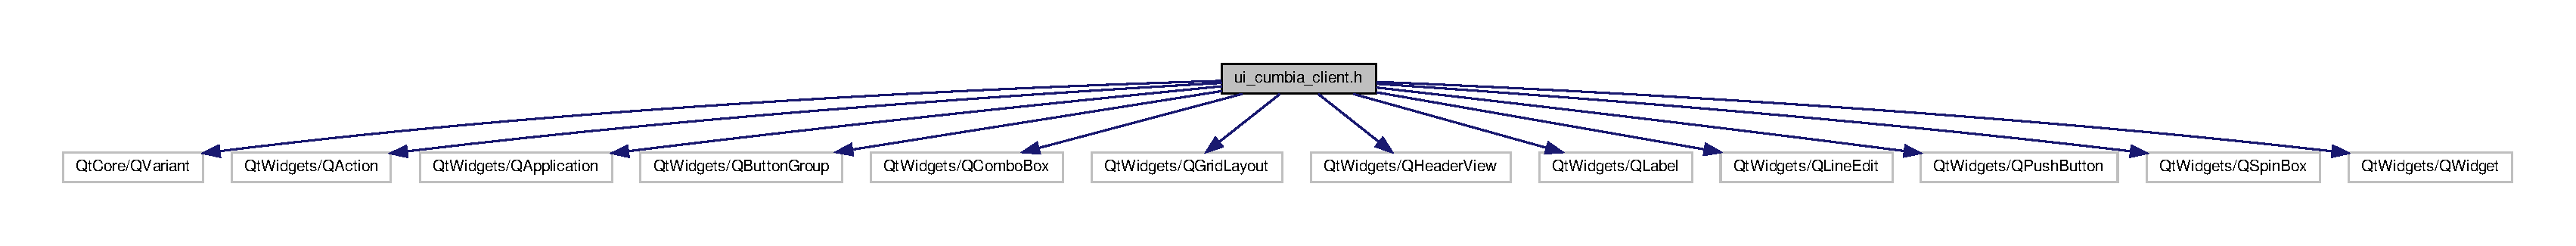
\includegraphics[width=350pt]{ui__cumbia__client_8h__incl}
\end{center}
\end{figure}

\input{ui__qumbia-client_8h}
%--- End generated contents ---

% Index
\backmatter
\newpage
\phantomsection
\clearemptydoublepage
\addcontentsline{toc}{chapter}{Index}
\printindex

\end{document}
